% document type
\documentclass[12pt]{article}

% packages
\usepackage[total={170mm,230mm}]{geometry}
\usepackage[utf8]{inputenc}
\usepackage[T1]{fontenc}
\usepackage[russian]{babel}
\usepackage{graphicx}
\usepackage{amssymb}
\usepackage{amsfonts}
\usepackage{amsmath}
\usepackage{amsthm}
\usepackage{physics}
\usepackage{nicefrac}
\usepackage{cancel}
\usepackage{hyperref}
\usepackage{cmap}

\title{Опыт Франка\---Герца}
\author{Козлов Александр \and Краснощёкова Дарья}

\begin{document}
	%!TEX root = ../diode.tex
\begin{titlepage}
	\begin{center}
	% \vspace{-3em}
	{\small\textsc{Нижегородский государственный университет имени Н.\,И. Лобачевского}}
	\vskip 2pt \hrule \vskip 3pt
	{\small\textsc{Высшая школа общей и прикладной физики}}

	\vfill


	{{\large Отчет по лабораторной работе}\vskip 12 pt {\Large \bfseries Эффект Зеемана}}

		
	\vspace{2cm}
	{\large Работу выполнили студенты \\[0.5em]{\Large \bfseries Краснощёкова Дарья, Козлов Александр}}

	\end{center}

	\vfill

	\begin{center}
	{Нижний Новгород, \today}
	\end{center}
\end{titlepage}

	\tableofcontents
	\newpage
	\section{Определение резонансного потенциала}
	Сняли анодно\---сеточную характеристику при задерживающем напряжении, при котором видно два максимума анодно\---сеточной характеристики наилучшим образом. Задерживающее напряжение было выбрано $7.5\ \text{В}$. Напряжение накала выставили $3\ \text{В}$. Результаты измерений отображены на рисунке \ref{fig:figure1}.
	\begin{figure}[htbp]
		\centering
		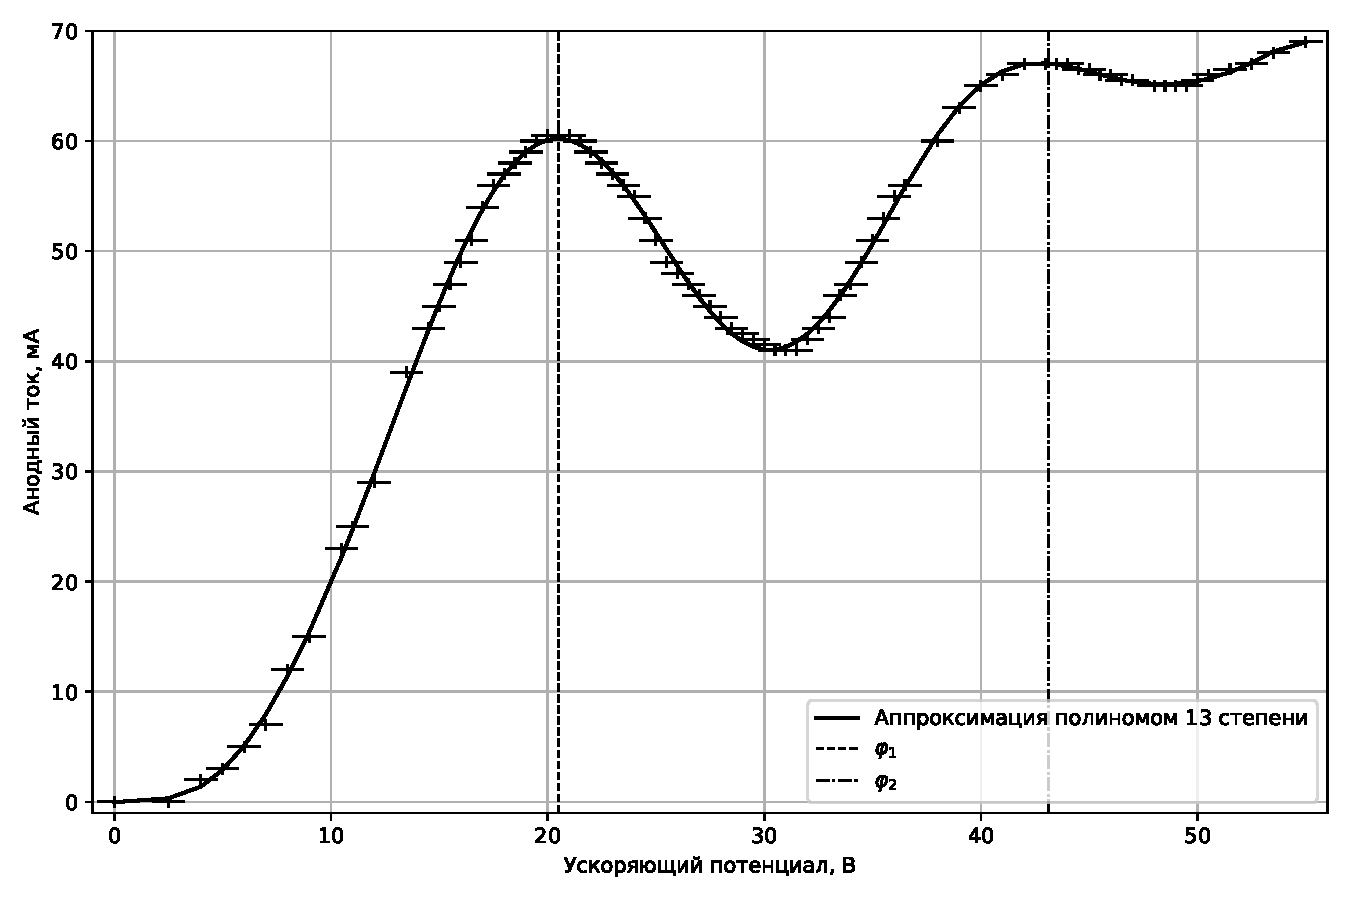
\includegraphics[width=\linewidth]{../plots/1}
		\caption{Анодно-сеточная характеристика при задерживающем напряжении $7.5\ \text{В}$ и напряжении накала $3\ \text{В}$.}
		\label{fig:figure1}
	\end{figure}
	Первые два локальных максимума обнаружены при ускоряющих потенциалах $\varphi_1 = 20.50\pm0.85\ \text{В}$ и $\varphi_2 = 43.13\pm1.05\ \text{В}$.
	\par Наиболее близко к табличному значению резонансного потенциала для гелия, которое составляет $21\ \text{В}$, значение потенциала, отвечающее первому максимому анодно-сеточной характеристики. Разность 
	\begin{equation}
		\varphi_2 - \varphi_1 = 22.63\pm1.90\ \text{В}
	\end{equation}
	сильнее отличается от табличного значения, хотя последнее захватывается интервалом погрешности данной величины. Выбрав наиболее близкое к табличному значение резонансного потенциала, находим разность энергий
	\begin{equation}
			E_1 - E_0 = eV_\text{рез} = 20.50\pm0.85\ \text{эВ}.
	\end{equation}

	\section{Определение потенциала ионизации}
	Для определения потенциала ионизации искали скачок анодного тока при потенциале задержки, большем ускоряющего потенциала. Провели три серии измерений с различными потенциалами задержки. Результаты измерений представлены на рисунке \ref{fig:figure2}.
	\begin{figure}[htbp]
		\centering
		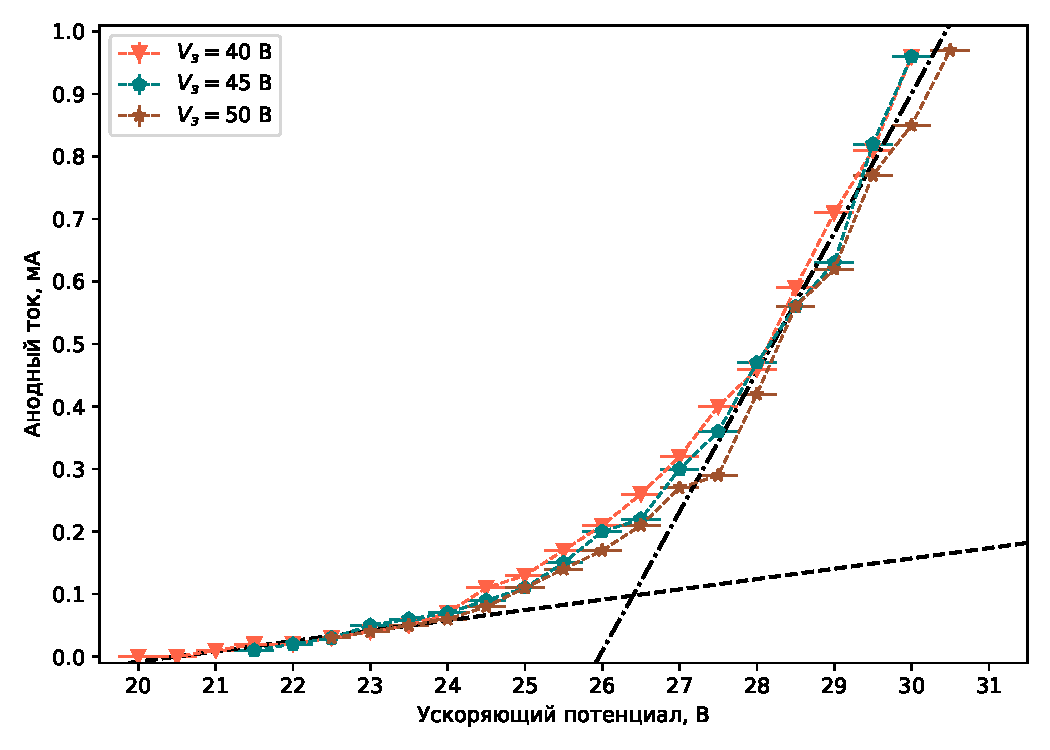
\includegraphics[width=\linewidth]{../plots/2}
		\caption{Анодно-сеточная характеристика при потенциалах задержки $40$, $45$ и $50$ вольт. Пунктирными линиями обозначены линейные аппроксимации комбинированного графика до и после ионизации.}
		\label{fig:figure2}
	\end{figure}
	Из графика видно, что скачок производной достаточно сильно размазан и находится в интервале ускоряющих потенциалов от $24\ \text{В}$ до $27\ \text{В}$. Следовательно, потенциал ионизации возможно определить так:
	\begin{equation}
		\varphi_\text{и} = 25.5\pm1.5\ \text{В}.
	\end{equation}
	\par Потенциал ионизации, определённый нами, с учётом погрешности хорошо совпадает с действительным, который составляет $24.5\ \text{В}$.
\end{document}